%%
% Copyright (c) 2017 - 2021, Pascal Wagler;
% Copyright (c) 2014 - 2021, John MacFarlane
%
% All rights reserved.
%
% Redistribution and use in source and binary forms, with or without
% modification, are permitted provided that the following conditions
% are met:
%
% - Redistributions of source code must retain the above copyright
% notice, this list of conditions and the following disclaimer.
%
% - Redistributions in binary form must reproduce the above copyright
% notice, this list of conditions and the following disclaimer in the
% documentation and/or other materials provided with the distribution.
%
% - Neither the name of John MacFarlane nor the names of other
% contributors may be used to endorse or promote products derived
% from this software without specific prior written permission.
%
% THIS SOFTWARE IS PROVIDED BY THE COPYRIGHT HOLDERS AND CONTRIBUTORS
% "AS IS" AND ANY EXPRESS OR IMPLIED WARRANTIES, INCLUDING, BUT NOT
% LIMITED TO, THE IMPLIED WARRANTIES OF MERCHANTABILITY AND FITNESS
% FOR A PARTICULAR PURPOSE ARE DISCLAIMED. IN NO EVENT SHALL THE
% COPYRIGHT OWNER OR CONTRIBUTORS BE LIABLE FOR ANY DIRECT, INDIRECT,
% INCIDENTAL, SPECIAL, EXEMPLARY, OR CONSEQUENTIAL DAMAGES (INCLUDING,
% BUT NOT LIMITED TO, PROCUREMENT OF SUBSTITUTE GOODS OR SERVICES;
% LOSS OF USE, DATA, OR PROFITS; OR BUSINESS INTERRUPTION) HOWEVER
% CAUSED AND ON ANY THEORY OF LIABILITY, WHETHER IN CONTRACT, STRICT
% LIABILITY, OR TORT (INCLUDING NEGLIGENCE OR OTHERWISE) ARISING IN
% ANY WAY OUT OF THE USE OF THIS SOFTWARE, EVEN IF ADVISED OF THE
% POSSIBILITY OF SUCH DAMAGE.
%%

%%
% This is the Eisvogel pandoc LaTeX template.
%
% For usage information and examples visit the official GitHub page:
% https://github.com/Wandmalfarbe/pandoc-latex-template
%%

% Options for packages loaded elsewhere
\PassOptionsToPackage{unicode}{hyperref}
\PassOptionsToPackage{hyphens}{url}
\PassOptionsToPackage{dvipsnames,svgnames*,x11names*,table}{xcolor}
%
\documentclass[
  english,
  paper=a4,
  oneside  ,captions=tableheading
]{scrbook}
\usepackage{amsmath,amssymb}
\usepackage{lmodern}
\usepackage{setspace}
\setstretch{1.2}
\usepackage{ifxetex,ifluatex}
\ifnum 0\ifxetex 1\fi\ifluatex 1\fi=0 % if pdftex
  \usepackage[T1]{fontenc}
  \usepackage[utf8]{inputenc}
  \usepackage{textcomp} % provide euro and other symbols
\else % if luatex or xetex
  \usepackage{unicode-math}
  \defaultfontfeatures{Scale=MatchLowercase}
  \defaultfontfeatures[\rmfamily]{Ligatures=TeX,Scale=1}
\fi
% Use upquote if available, for straight quotes in verbatim environments
\IfFileExists{upquote.sty}{\usepackage{upquote}}{}
\IfFileExists{microtype.sty}{% use microtype if available
  \usepackage[]{microtype}
  \UseMicrotypeSet[protrusion]{basicmath} % disable protrusion for tt fonts
}{}
\makeatletter
\@ifundefined{KOMAClassName}{% if non-KOMA class
  \IfFileExists{parskip.sty}{%
    \usepackage{parskip}
  }{% else
    \setlength{\parindent}{0pt}
    \setlength{\parskip}{6pt plus 2pt minus 1pt}}
}{% if KOMA class
  \KOMAoptions{parskip=half}}
\makeatother
\usepackage{fancyvrb}
\usepackage{xcolor}
\definecolor{default-linkcolor}{HTML}{A50000}
\definecolor{default-filecolor}{HTML}{A50000}
\definecolor{default-citecolor}{HTML}{4077C0}
\definecolor{default-urlcolor}{HTML}{4077C0}
\IfFileExists{xurl.sty}{\usepackage{xurl}}{} % add URL line breaks if available
\IfFileExists{bookmark.sty}{\usepackage{bookmark}}{\usepackage{hyperref}}
\hypersetup{
  pdftitle={Project Requirements, Plan and Task Definitions},
  pdfauthor={Callum Stewart; Saad Badshah; Abigail Rivera; Daniel Scott; Bruce Wilson; Sebastian Zebrowski},
  pdflang={en},
  hidelinks,
  breaklinks=true,
  pdfcreator={LaTeX via pandoc with the Eisvogel template}}
\urlstyle{same} % disable monospaced font for URLs
\VerbatimFootnotes % allow verbatim text in footnotes
\usepackage[margin=2.5cm,includehead=true,includefoot=true,centering,]{geometry}
\usepackage{listings}
\newcommand{\passthrough}[1]{#1}
\lstset{defaultdialect=[5.3]Lua}
\lstset{defaultdialect=[x86masm]Assembler}
\usepackage{longtable,booktabs,array}
\usepackage{calc} % for calculating minipage widths
% Correct order of tables after \paragraph or \subparagraph
\usepackage{etoolbox}
\makeatletter
\patchcmd\longtable{\par}{\if@noskipsec\mbox{}\fi\par}{}{}
\makeatother
% Allow footnotes in longtable head/foot
\IfFileExists{footnotehyper.sty}{\usepackage{footnotehyper}}{\usepackage{footnote}}
\makesavenoteenv{longtable}
% add backlinks to footnote references, cf. https://tex.stackexchange.com/questions/302266/make-footnote-clickable-both-ways
\usepackage{footnotebackref}
\usepackage{graphicx}
\makeatletter
\def\maxwidth{\ifdim\Gin@nat@width>\linewidth\linewidth\else\Gin@nat@width\fi}
\def\maxheight{\ifdim\Gin@nat@height>\textheight\textheight\else\Gin@nat@height\fi}
\makeatother
% Scale images if necessary, so that they will not overflow the page
% margins by default, and it is still possible to overwrite the defaults
% using explicit options in \includegraphics[width, height, ...]{}
\setkeys{Gin}{width=\maxwidth,height=\maxheight,keepaspectratio}
% Set default figure placement to htbp
\makeatletter
\def\fps@figure{htbp}
\makeatother
\setlength{\emergencystretch}{3em} % prevent overfull lines
\providecommand{\tightlist}{%
  \setlength{\itemsep}{0pt}\setlength{\parskip}{0pt}}
\setcounter{secnumdepth}{-\maxdimen} % remove section numbering

% Make use of float-package and set default placement for figures to H.
% The option H means 'PUT IT HERE' (as  opposed to the standard h option which means 'You may put it here if you like').
\usepackage{float}
\floatplacement{figure}{H}

\ifxetex
    % See issue https://github.com/reutenauer/polyglossia/issues/127
  \renewcommand*\familydefault{\sfdefault}
    % Load polyglossia as late as possible: uses bidi with RTL langages (e.g. Hebrew, Arabic)
  \usepackage{polyglossia}
  \setmainlanguage[]{}
\else
  \usepackage[main=english]{babel}
% get rid of language-specific shorthands (see #6817):
\let\LanguageShortHands\languageshorthands
\def\languageshorthands#1{}
\fi
\ifluatex
  \usepackage{selnolig}  % disable illegal ligatures
\fi

\title{Project Requirements, Plan and Task Definitions}
\usepackage{etoolbox}
\makeatletter
\providecommand{\subtitle}[1]{% add subtitle to \maketitle
  \apptocmd{\@title}{\par {\large #1 \par}}{}{}
}
\makeatother
\subtitle{Deliverable 1 Report}
\author{Callum Stewart \and Saad Badshah \and Abigail Rivera \and Daniel
Scott \and Bruce Wilson \and Sebastian Zebrowski}
\date{2021-01-31}



%%
%% added
%%

%
% language specification
%
% If no language is specified, use English as the default main document language.
%



%
% for the background color of the title page
%
\usepackage{pagecolor}
\usepackage{afterpage}
\usepackage[margin=2.5cm,includehead=true,includefoot=true,centering]{geometry}

%
% break urls
%
\PassOptionsToPackage{hyphens}{url}

%
% When using babel or polyglossia with biblatex, loading csquotes is recommended
% to ensure that quoted texts are typeset according to the rules of your main language.
%
\usepackage{csquotes}

%
% captions
%
\definecolor{caption-color}{HTML}{777777}
\usepackage[font={stretch=1.2}, textfont={color=caption-color}, position=top, skip=4mm, labelfont=bf, singlelinecheck=false, justification=raggedright]{caption}
\setcapindent{0em}

%
% blockquote
%
\definecolor{blockquote-border}{RGB}{221,221,221}
\definecolor{blockquote-text}{RGB}{119,119,119}
\usepackage{mdframed}
\newmdenv[rightline=false,bottomline=false,topline=false,linewidth=3pt,linecolor=blockquote-border,skipabove=\parskip]{customblockquote}
\renewenvironment{quote}{\begin{customblockquote}\list{}{\rightmargin=0em\leftmargin=0em}%
\item\relax\color{blockquote-text}\ignorespaces}{\unskip\unskip\endlist\end{customblockquote}}

%
% Source Sans Pro as the de­fault font fam­ily
% Source Code Pro for monospace text
%
% 'default' option sets the default
% font family to Source Sans Pro, not \sfdefault.
%
\ifnum 0\ifxetex 1\fi\ifluatex 1\fi=0 % if pdftex
    \usepackage[default]{sourcesanspro}
  \usepackage{sourcecodepro}
  \else % if not pdftex
    \usepackage[default]{sourcesanspro}
  \usepackage{sourcecodepro}

  % XeLaTeX specific adjustments for straight quotes: https://tex.stackexchange.com/a/354887
  % This issue is already fixed (see https://github.com/silkeh/latex-sourcecodepro/pull/5) but the
  % fix is still unreleased.
  % TODO: Remove this workaround when the new version of sourcecodepro is released on CTAN.
  \ifxetex
    \makeatletter
    \defaultfontfeatures[\ttfamily]
      { Numbers   = \sourcecodepro@figurestyle,
        Scale     = \SourceCodePro@scale,
        Extension = .otf }
    \setmonofont
      [ UprightFont    = *-\sourcecodepro@regstyle,
        ItalicFont     = *-\sourcecodepro@regstyle It,
        BoldFont       = *-\sourcecodepro@boldstyle,
        BoldItalicFont = *-\sourcecodepro@boldstyle It ]
      {SourceCodePro}
    \makeatother
  \fi
  \fi

%
% heading color
%
\definecolor{heading-color}{RGB}{40,40,40}
\addtokomafont{section}{\color{heading-color}}
% When using the classes report, scrreprt, book,
% scrbook or memoir, uncomment the following line.
%\addtokomafont{chapter}{\color{heading-color}}

%
% variables for title, author and date
%
\usepackage{titling}
\title{Project Requirements, Plan and Task Definitions}
\author{Callum Stewart, Saad Badshah, Abigail Rivera, Daniel
Scott, Bruce Wilson, Sebastian Zebrowski}
\date{2021-01-31}

%
% tables
%

\definecolor{table-row-color}{HTML}{F5F5F5}
\definecolor{table-rule-color}{HTML}{999999}

%\arrayrulecolor{black!40}
\arrayrulecolor{table-rule-color}     % color of \toprule, \midrule, \bottomrule
\setlength\heavyrulewidth{0.3ex}      % thickness of \toprule, \bottomrule
\renewcommand{\arraystretch}{1.3}     % spacing (padding)


%
% remove paragraph indention
%
\setlength{\parindent}{0pt}
\setlength{\parskip}{6pt plus 2pt minus 1pt}
\setlength{\emergencystretch}{3em}  % prevent overfull lines

%
%
% Listings
%
%


%
% general listing colors
%
\definecolor{listing-background}{HTML}{F7F7F7}
\definecolor{listing-rule}{HTML}{B3B2B3}
\definecolor{listing-numbers}{HTML}{B3B2B3}
\definecolor{listing-text-color}{HTML}{000000}
\definecolor{listing-keyword}{HTML}{435489}
\definecolor{listing-keyword-2}{HTML}{1284CA} % additional keywords
\definecolor{listing-keyword-3}{HTML}{9137CB} % additional keywords
\definecolor{listing-identifier}{HTML}{435489}
\definecolor{listing-string}{HTML}{00999A}
\definecolor{listing-comment}{HTML}{8E8E8E}

\lstdefinestyle{eisvogel_listing_style}{
  language         = java,
  numbers          = left,
  xleftmargin      = 2.7em,
  framexleftmargin = 2.5em,
  backgroundcolor  = \color{listing-background},
  basicstyle       = \color{listing-text-color}\linespread{1.0}\scriptsize\ttfamily{},
  breaklines       = true,
  frame            = single,
  framesep         = 0.19em,
  rulecolor        = \color{listing-rule},
  frameround       = ffff,
  tabsize          = 4,
  numberstyle      = \color{listing-numbers},
  aboveskip        = 1.0em,
  belowskip        = 0.1em,
  abovecaptionskip = 0em,
  belowcaptionskip = 1.0em,
  keywordstyle     = {\color{listing-keyword}\bfseries},
  keywordstyle     = {[2]\color{listing-keyword-2}\bfseries},
  keywordstyle     = {[3]\color{listing-keyword-3}\bfseries\itshape},
  sensitive        = true,
  identifierstyle  = \color{listing-identifier},
  commentstyle     = \color{listing-comment},
  stringstyle      = \color{listing-string},
  showstringspaces = false,
  escapeinside     = {/*@}{@*/}, % Allow LaTeX inside these special comments
  literate         =
  {á}{{\'a}}1 {é}{{\'e}}1 {í}{{\'i}}1 {ó}{{\'o}}1 {ú}{{\'u}}1
  {Á}{{\'A}}1 {É}{{\'E}}1 {Í}{{\'I}}1 {Ó}{{\'O}}1 {Ú}{{\'U}}1
  {à}{{\`a}}1 {è}{{\'e}}1 {ì}{{\`i}}1 {ò}{{\`o}}1 {ù}{{\`u}}1
  {À}{{\`A}}1 {È}{{\'E}}1 {Ì}{{\`I}}1 {Ò}{{\`O}}1 {Ù}{{\`U}}1
  {ä}{{\"a}}1 {ë}{{\"e}}1 {ï}{{\"i}}1 {ö}{{\"o}}1 {ü}{{\"u}}1
  {Ä}{{\"A}}1 {Ë}{{\"E}}1 {Ï}{{\"I}}1 {Ö}{{\"O}}1 {Ü}{{\"U}}1
  {â}{{\^a}}1 {ê}{{\^e}}1 {î}{{\^i}}1 {ô}{{\^o}}1 {û}{{\^u}}1
  {Â}{{\^A}}1 {Ê}{{\^E}}1 {Î}{{\^I}}1 {Ô}{{\^O}}1 {Û}{{\^U}}1
  {œ}{{\oe}}1 {Œ}{{\OE}}1 {æ}{{\ae}}1 {Æ}{{\AE}}1 {ß}{{\ss}}1
  {ç}{{\c c}}1 {Ç}{{\c C}}1 {ø}{{\o}}1 {å}{{\r a}}1 {Å}{{\r A}}1
  {€}{{\EUR}}1 {£}{{\pounds}}1 {«}{{\guillemotleft}}1
  {»}{{\guillemotright}}1 {ñ}{{\~n}}1 {Ñ}{{\~N}}1 {¿}{{?`}}1
  {…}{{\ldots}}1 {≥}{{>=}}1 {≤}{{<=}}1 {„}{{\glqq}}1 {“}{{\grqq}}1
  {”}{{''}}1
}
\lstset{style=eisvogel_listing_style}

%
% Java (Java SE 12, 2019-06-22)
%
\lstdefinelanguage{Java}{
  morekeywords={
    % normal keywords (without data types)
    abstract,assert,break,case,catch,class,continue,default,
    do,else,enum,exports,extends,final,finally,for,if,implements,
    import,instanceof,interface,module,native,new,package,private,
    protected,public,requires,return,static,strictfp,super,switch,
    synchronized,this,throw,throws,transient,try,volatile,while,
    % var is an identifier
    var
  },
  morekeywords={[2] % data types
    % primitive data types
    boolean,byte,char,double,float,int,long,short,
    % String
    String,
    % primitive wrapper types
    Boolean,Byte,Character,Double,Float,Integer,Long,Short
    % number types
    Number,AtomicInteger,AtomicLong,BigDecimal,BigInteger,DoubleAccumulator,DoubleAdder,LongAccumulator,LongAdder,Short,
    % other
    Object,Void,void
  },
  morekeywords={[3] % literals
    % reserved words for literal values
    null,true,false,
  },
  sensitive,
  morecomment  = [l]//,
  morecomment  = [s]{/*}{*/},
  morecomment  = [s]{/**}{*/},
  morestring   = [b]",
  morestring   = [b]',
}

\lstdefinelanguage{XML}{
  morestring      = [b]",
  moredelim       = [s][\bfseries\color{listing-keyword}]{<}{\ },
  moredelim       = [s][\bfseries\color{listing-keyword}]{</}{>},
  moredelim       = [l][\bfseries\color{listing-keyword}]{/>},
  moredelim       = [l][\bfseries\color{listing-keyword}]{>},
  morecomment     = [s]{<?}{?>},
  morecomment     = [s]{<!--}{-->},
  commentstyle    = \color{listing-comment},
  stringstyle     = \color{listing-string},
  identifierstyle = \color{listing-identifier}
}

%
% header and footer
%
\usepackage{fancyhdr}

\fancypagestyle{eisvogel-header-footer}{
  \fancyhead{}
  \fancyfoot{}
  \lhead[2021-01-31]{Project Requirements, Plan and Task Definitions}
  \chead[]{}
  \rhead[Project Requirements, Plan and Task Definitions]{2021-01-31}
  \lfoot[\thepage]{Callum Stewart, Saad Badshah, Abigail Rivera, Daniel
Scott, Bruce Wilson, Sebastian Zebrowski}
  \cfoot[]{}
  \rfoot[Callum Stewart, Saad Badshah, Abigail Rivera, Daniel
Scott, Bruce Wilson, Sebastian Zebrowski]{\thepage}
  \renewcommand{\headrulewidth}{0.4pt}
  \renewcommand{\footrulewidth}{0.4pt}
}
\pagestyle{eisvogel-header-footer}

%%
%% end added
%%

\begin{document}

%%
%% begin titlepage
%%
\begin{titlepage}
\newgeometry{left=6cm}
\definecolor{titlepage-color}{HTML}{483D8B}
\newpagecolor{titlepage-color}\afterpage{\restorepagecolor}
\newcommand{\colorRule}[3][black]{\textcolor[HTML]{#1}{\rule{#2}{#3}}}
\begin{flushleft}
\noindent
\\[-1em]
\color[HTML]{FFFAFA}
\makebox[0pt][l]{\colorRule[FFFAFA]{1.3\textwidth}{2pt}}
\par
\noindent

{
  \setstretch{1.4}
  \vfill
  \noindent {\huge \textbf{\textsf{Project Requirements, Plan and Task
Definitions}}}
    \vskip 1em
  {\Large \textsf{Deliverable 1 Report}}
    \vskip 2em
  \noindent {\Large \textsf{Callum Stewart, Saad Badshah, Abigail
Rivera, Daniel Scott, Bruce Wilson, Sebastian Zebrowski}}
  \vfill
}


\textsf{2021-01-31}
\end{flushleft}
\end{titlepage}
\restoregeometry

%%
%% end titlepage
%%


\hypertarget{background-and-motivation}{%
\section{Background and Motivation}\label{background-and-motivation}}

\hypertarget{motivation}{%
\subsection{Motivation}\label{motivation}}

In this project we are seeking to create an educational tool that can be
used to interactively explore the differences between two approaches to
time series analysis of non-stationary signals. The front end only
application will allow users to either submit their own signals, or to
build one using a library of predefined signal types, and then perform
either a Short Time Fourier Transform or a Empirical Mode Decomposition
on the signal to break it down into it's constituent component signals.

This will allow them to explore the differences between these two
methods for decomposing time signals, serving as a demonstration of
their relative strengths and weakness, and providing an intuitive feel
for how they work. The application will also have a number of
convenience features for users, such as the ability to bookmark
examples, and a pre-generated set of examples that can be used to
demonstrate how the application and how the time series analysis
techniques work.

\hypertarget{background}{%
\subsection{Background}\label{background}}

\hypertarget{time-series-analysis}{%
\subsubsection{Time Series Analysis}\label{time-series-analysis}}

A \emph{time series} is a sequence of data points that are indexed or
graphed in time order. Frequently graphed in a run chart (a graph which
features time as its \(`y`\) axis), time series occur naturally in a
wide array of subjects, such as statistics, finance, weather
forecasting, and signal processing.

There are a handful of common types of time series that occur widely,
for example: 1. Simple sinusoids 1. Linear, exponential, logarithmic, or
polynomial trends 1. White, coloured, or shot noise 1. Chirps 1.
Products and sums of the above signals, forming complex signals that
might be found in the real world

\emph{Time series analysis} is a set of techniques that can be used in
order to reason about time series', enabling an analyst to extract
useful insights from the data.

Many time series exhibit an oscillatory behaviour, such as the
temperature of a city on any given day of the year, the share price of a
given stock, or the audio data recorded by a microphone. An analyst can
exploit the fact that complex signals can be approximated with sums of
simpler trigonometric functions and use Fourier analysis to decompose a
signal into its oscillatory components.

\hypertarget{discrete-fourier-transform}{%
\subsubsection{Discrete Fourier
Transform}\label{discrete-fourier-transform}}

\begin{figure}
\centering
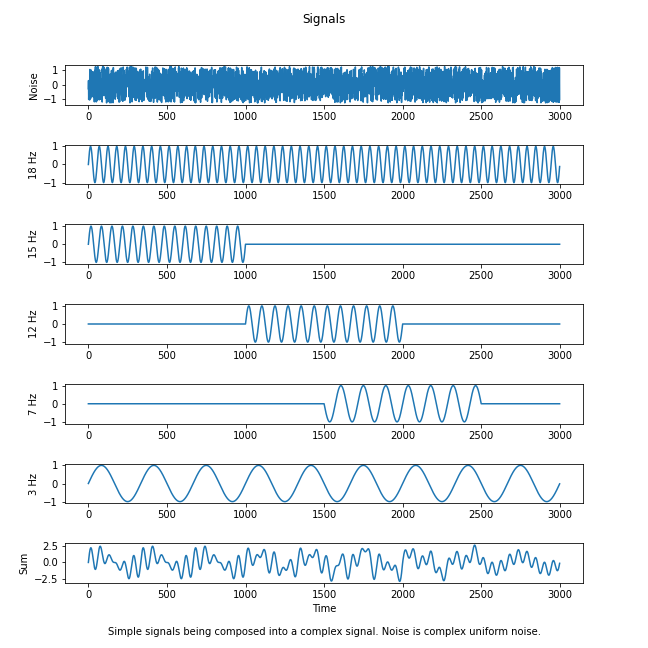
\includegraphics{img/composite_signal.png}
\caption{Complex signal derived from simple signals}
\end{figure}

A Fourier transform is one way of decomposing a complex signal into its
oscillatory components, revealing the frequencies of the constituent
component signals. Determining what component frequencies are present in
a signal can give an insight into the nature of a signal, or allow it to
be manipulated precisely. For example, it may allow an audio engineer to
silence or boost particular frequencies as they see fit, or a financial
analyst to determine what kind of long term trends exist in financial
data. Lets look at an example of a Fourier transform of the previous
signal. We will use the Fast Fourier Transform (FFT) algorithm to
compute the transform.

\begin{figure}
\centering
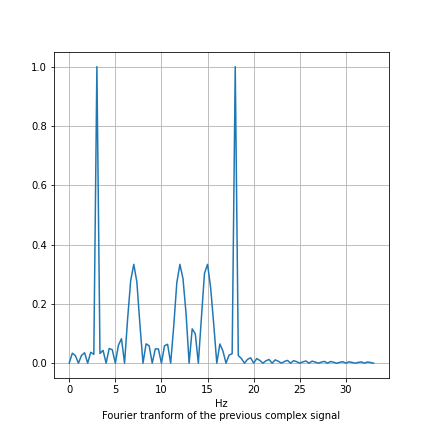
\includegraphics{img/fft.png}
\caption{Fourier transform of complex signal}
\end{figure}

Notice that despite having a strong indication that the constant 3Hz and
18Hz signals are constituent components, much information has been lost.
As a Fourier transform maps a function from the time domain to the
frequency domain, all temporal information is lost, as the FFT assumes
periodicity. This is obviously not ideal, as our complex signal is
non-linear. The Fourier transform is thus not well suited to non-linear
signals when applied on the entire signal at once.

\hypertarget{short-time-fourier-transform}{%
\subsubsection{Short Time Fourier
Transform}\label{short-time-fourier-transform}}

Instead, in order to study non-stationary signals, we require a
technique that can study a signal in both the time and frequency domain
simultaneously. The simplest of these techniques is the Short Time
Fourier Transform (STFT).

The procedure for STFT is to divide a long time signal equally into
shorter length segments, and then compute a DFT on each of these
segments. In order to smooth out any unusual artefacts at the boundary
of segments, window functions such as a Hann window may be used, which
attenuates signals located near boundaries using a cosine window. With
the Fourier spectra of each shorter segment, we can plot the changing
spectra against time using a type of plot known as a spectrogram. Here
is an example of STFT applied to our original signal.

\begin{figure}
\centering
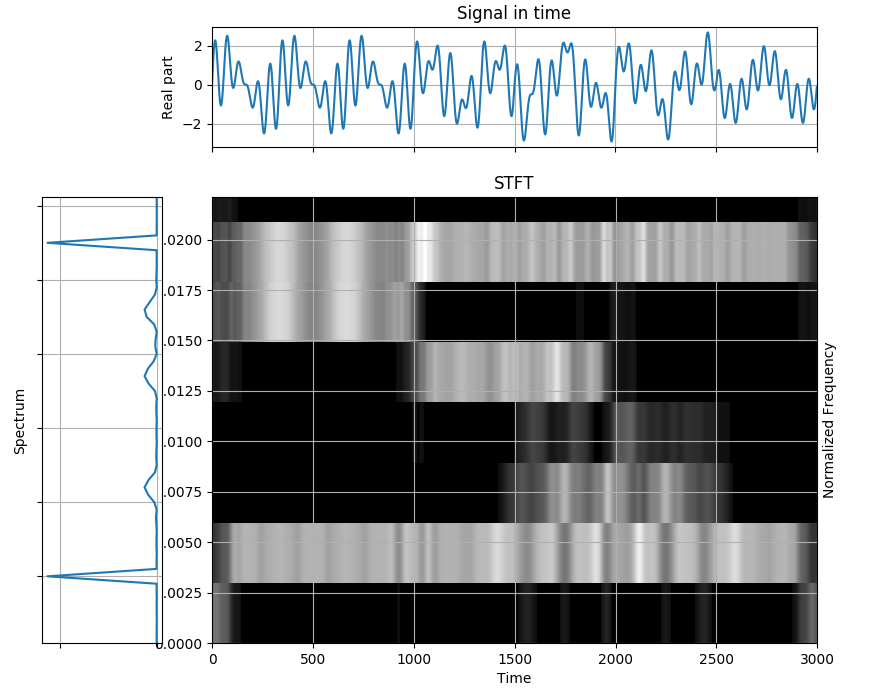
\includegraphics{img/stft_output_spectra.png}
\caption{Resulting spectra from STFT applied to complex signal}
\end{figure}

Here we can see the strength of each constituent signal by colour
intensity. Unlike previously with the FFT, we now have temporal
information, and can see when signals of a given frequency begin and end
in the complex signal.

However there is a significant limitation to building on top of Fourier
transforms due to an uncertainty limit called the Gabor limit. By making
the time resolution smaller (i.e., by dividing the main signal into
smaller windows) we become more certain of when frequencies change, but
we lose frequency resolution (the ability to see frequency components
close together). By making the time resolutions larger, we lose time
resolution (the ability to know precisely when a frequency changes), but
we get better frequency resolution.

\hypertarget{hilbert-huang-transform-and-empirical-mode-decomposition}{%
\subsubsection{Hilbert-Huang Transform and Empirical Mode
Decomposition}\label{hilbert-huang-transform-and-empirical-mode-decomposition}}

The Hilbert-Huang Transform (HHT) is a powerful time-frequency analysis
technique. It allows an analyst to decompose a complex signal into a
number of orthogonal Intrinsic Mode Frequencies (IMFs) with a trend
using EMD and applies Hilbert Spectral Analysis (HSA) to the IMFs to
obtain information regarding instantaneous frequency.

HHT first utilises empirical mode decomposition (EMD) in order to break
a complex waveform into IMFs representing simple oscillatory modes
through a process called sifting. The amplitude and frequency of an IMF
may vary with time, and must satisfy both of these rules: 1. The total
number of extrema and the number of zero crossings must differ by at
most 1 2. The mean envelope value (defined by a spline described by the
local maxima and the local minima) must be nearly zero

The sifting procedure to extract these IMFs can be described by the
following steps: 1. Initialise \(`r_0 = X(t)`\) and \(`i = 1`\) 1. Start
outer loop 1. Extract the \(`i`\)th IMF \(`c_i`\) 1. Initialise
\(`h_{k(k-1)} = r_{i-1}`\), \(`k = 1`\) 1. Start inner loop 1. Identify
all of the local maxima and minima (the extrema) 1. Interpolate the
minima with a cubic spline in order to define the lower envelope 1.
Interpolate the maxima with a cubic spline in order to define the upper
envelope 1. Calculate the mean \(`m_{i(k-1)}`\) of the upper and lower
envelopes of \(`h_{i(k-1)}`\). The envelope defined by the two cubic
splines should contain all data. 1. Set
\(`h_{ik} = h_{i(k-1)} - m_{i(k-1)}`\) 1. Is \(`h_{ik}`\) an IMF? - If
true, set \(`c_i = h_{ik}`\) and break - Else increment \(`k`\) and
continue inner loop 1. Set the remainder \(`r_{i+1} = r_i - c_i`\) 1.
Does \(`r_{i + 1}`\) contain at least two extrema? - If true increment
\(`i`\) and continue outer loop - Else end routine, with \(`r_{i + 1}`\)
as the signal residue and \(`c_1`\) through \(`c_i`\) as the IMFs

Below is a flowchart describing this algorithm\footnote{Lei, Yaguo, et
  al.~``A review on empirical mode decomposition in fault diagnosis of
  rotating machinery.'' \emph{Mechanical systems and signal processing
  35.1-2} (2013): 108-126.}

\begin{figure}
\centering
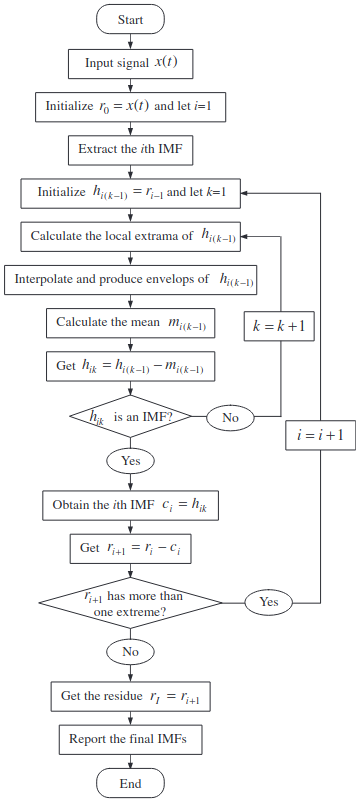
\includegraphics{img/emd_flowchart.png}
\caption{Flowchart of EMD algorithm}
\end{figure}

And below is an animation of the production of an IMF\footnote{Photograph
  by Geir Kulia and modified by Matt Hall, distributed under a Creative
  Commons Attribution-ShareAlike 4.0 license.}

\begin{figure}
\centering
\includegraphics{img/Emd_example_lowres.gif}
\caption{Animation of the sifting procedure used in EMD}
\end{figure}

The number of sifting steps required to produce an IMF is determined by
the stopping criterion. There are a number of stopping criterion that
can be used for EMD, each with their own advantages and disadvantages.
The one proposed by Huang et al.~(1998) however is the `Standard
Deviation' method. For each point in time, the difference between the
current component and the previous component is calculated, squared,
divided by the square of the previous component evaluated at that point
in time, and summed.

\begin{lstlisting}
SD_{k}=\sum _{{t=0}}^{{T}}{\frac  {|h_{{k-1}}(t)-h_{k}(t)|^{2}}{h_{{k-1}}^{2}(t)}}
\end{lstlisting}

Once this value falls below a predetermined threshold, the sifting
process can be stopped.

There are other stopping criterion that may be used however, such as S
Number Criterion or Energy Difference Tracking.

Below we can see an example of EMD being performed on a complex signal,
breaking it down into its constituent modes in descending frequency
order\footnote{Example adapted from the Jupyter Notebook tutorials
  created by the developers of Python's \passthrough{\lstinline!emd!}
  library, available
  \href{https://emd.readthedocs.io/en/stable/_downloads/e47aacca40568b7bb056bd96535966c4/emd_tutorials_jupyter.zip}{here}}.

\begin{figure}
\centering
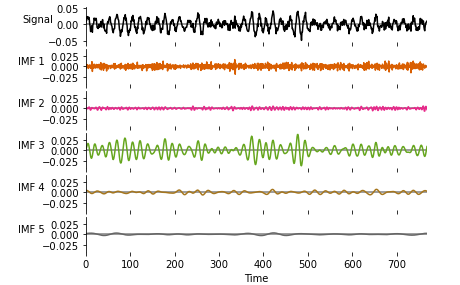
\includegraphics{img/emd_example.png}
\caption{An example of EMD being performed on a signal}
\end{figure}

At this point, if desired, the instantaneous frequency spectrum can be
obtained by applying the Hilbert transform on the constituent IMFs. The
final result would be called a Hilbert spectrum, where the amplitude and
instantaneous frequency can be plotted as functions of time on a three
dimensional plot.

Unlike STFT, EMD is a self-adaptive signal processing method. The IMFs
are determined by the signal itself, and are representative of the
natural oscillatory mode embedded in the signal. Thus EMD works on the
characteristic time local time scale, rather than with predetermined
windows.

Of course, EMD has weaknesses as well, for example:

\begin{enumerate}
\def\labelenumi{\arabic{enumi}.}
\tightlist
\item
  EMD suffers from end effects
\item
  The IMFs may not be orthogonal
\item
  Mode mixing sometimes occurs between IMFs, where a single IMF includes
  oscillatory modes that are drastically different or a component of a
  different IMF all together.
\end{enumerate}

In conclusion, each time-frequency analysis technique has draw backs and
advantages, and neither one is conclusively the correct one to use in
any given situation. This being said, for analysing non-stationary
signals EMD has some obvious advantages compared to STFT and can be
considered superior in most cases \footnote{Arun Raj P.D., Mr.~Venkatesh
  S., ``Time-Frequency Analysis methods: A Comparative study'',
  International Research Journal of Engineering and Technology
  (IRJET),Volume 3, Issue 6, June 2016, e-ISSN: 2395-0056.}.

\end{document}
